\chapter{Algoritmi Quantum Safe}

Per la stesura dell'elaborato sono stati considerati solo i sistemi di firma digitale presentati al NIST e, per specializzare maggiormente la ricerca, sono stati evitati i sistemi crittografici. Pur raggiungendo scopi diversi, sistemi di firma digitale e sistemi crittografici utilizzano la stessa teoria alla base. In generale, la Post-Quantum Cryptography (PQC), come la crittografia classica, si compone di algoritmi che sfruttano problemi o teoremi matematici complessi da risolvere con l’obiettivo di evitare la compromissione delle chiavi utilizzate per firmare o crittografare una o più comunicazioni. 

Nella PQC i problemi matematici devono essere difficili da risolvere sia per le tecnologie \textit{legacy} che per i computer quantistici, garantendo così la sicurezza contro attacchi avanzati. È fondamentale continuare a fare ricerca sui modelli già conosciuti e su nuovi modelli da utilizzare, poiché la loro sicurezza non è certificata. L'unico aspetto che si può affermare è che, con le conoscenze attuali, non sono noti attacchi in grado di compromettere facilmente tali schemi.

In questo elaborato verranno trattate solo le formulazioni matematiche più utilizzate per la creazione di algoritmi PQC. Analizzando i risultati del terzo \textit{round} del \textit{NIST Post-Quantum Cryptography Standardization Process} \cite{nist-pqc}, si nota che i finalisti appartengono principalmente a due classi di algoritmi PQC:
\begin{enumerate}
    \item CRYSTALS Dilithium: Lattice Based;
    \item FALCON: Lattice Based;
    \item SPHINCS+: Hash Based;
\end{enumerate}

Sebbene molte altre proposte, oltre a quelle elencate, utilizzino le stesse basi per creare sistemi crittografici o di firma digitale, esse sono tutte diverse. Gli algoritmi, pur partendo dalla stessa teoria matematica, possono essere differenziati dalle scelte implementative o dall'influenza di altri costrutti. Spesso, per la costruzione di un algoritmo di crittografia vengono combinati più problemi \textit{NP-Hard}, ovvero problemi notoriamente difficili da risolvere. L'originalità di questi algoritmi risiede nei problemi utilizzati e nel modo in cui essi sono interconnessi. La difficoltà \textit{NP-Hard} è cruciale per la sicurezza: questi schemi crittografici si affidano al fatto che, anche utilizzando un computer quantistico, risolvere tali problemi rimane computazionalmente proibitivo.

Nelle sezioni successive verranno esposte le idee alla base dei modelli presentati, senza eccessivi approfondimenti matematici, per rendere chiaro il contesto in cui operano questi algoritmi.

\section{Algoritmi basati su Lattice}

Dei quindici candidati iniziali del terzo \textit{round} del progetto NIST, sette utilizzano \textit{Lattice}. Ciò è dovuto alle caratteristiche intrinseche del problema, che è altamente configurabile e per il quale è dimostrato che sia i casi medi che quelli peggiori sono difficili da risolvere. I \textit{lattice based problems} rappresentano quindi una delle aree più promettenti e studiate nella crittografia post-quantistica.

Un \textit{lattice} (o reticolo) è un insieme di punti distribuiti regolarmente in uno spazio euclideo multidimensionale, generato da combinazioni lineari intere di un insieme di vettori linearmente indipendenti. Si può immaginare un \textit{lattice} come una griglia tridimensionale (o di dimensioni superiori) di punti, dove la posizione di ogni punto è determinata da combinazioni specifiche di alcuni vettori di base.

\begin{figure}[H]
    \centering
    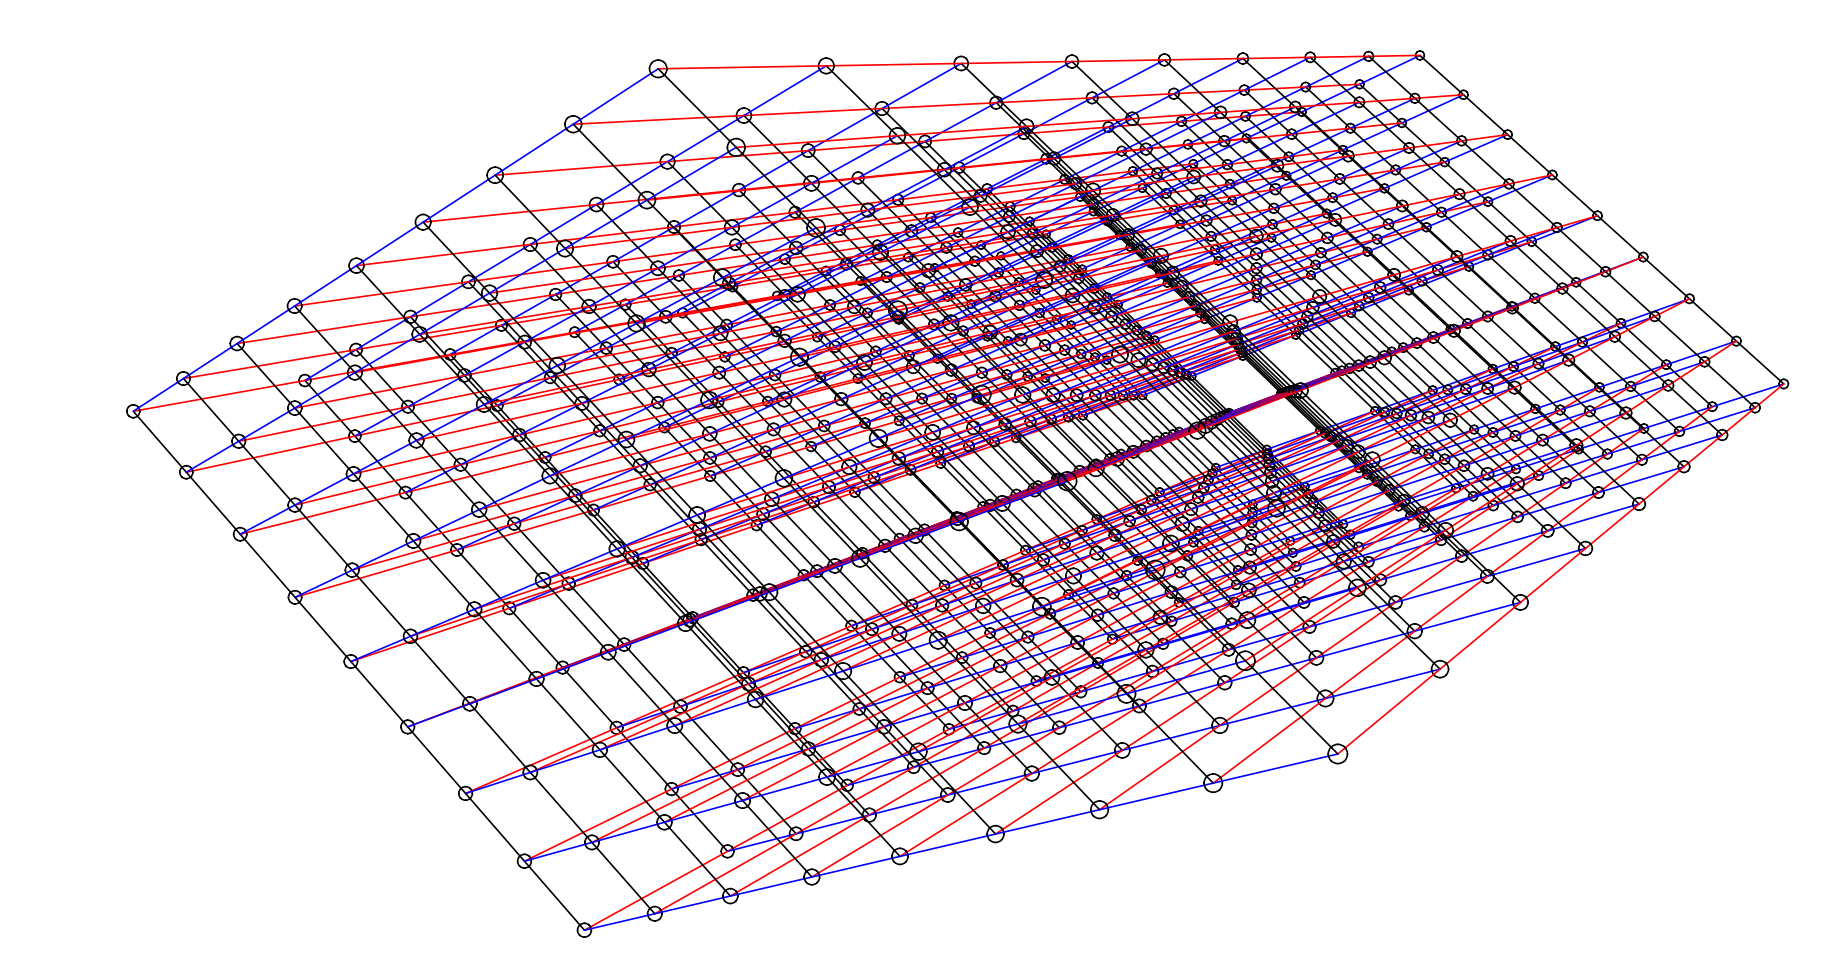
\includegraphics[width=0.8\textwidth]{Immagini/20240909_LBS.png}
    \caption{\textit{Lattice} tridimensionale basato su un sottoinsieme di 9x9x9 punti. Fonte: \cite{nature-pqc}}
\end{figure}

Nella crittografia basata su \textit{lattice}, la sicurezza degli schemi crittografici si basa sulla difficoltà di risolvere problemi matematici associati ai reticoli, come il problema del vettore più corto (\textit{Shortest Vector Problem}, SVP) e il problema del vettore più vicino (\textit{Closest Vector Problem}, CVP). Il problema SVP richiede di trovare il vettore non nullo più corto in un reticolo, mentre il CVP consiste nel trovare il punto del reticolo più vicino a un punto dato che non appartiene al reticolo stesso \cite{NISTthirdReport}. Entrambi questi problemi sono notoriamente difficili da risolvere, specialmente in spazi ad alta dimensione.

\subsection{Il Short Integer Solution Problem}

In particolare il problema alla base dei reticoli è stato definito da Ajtai nel 1996, il \textit{Short Integer Solution Problem (SIS)}:
\begin{displayquote}[NIST IR 8413, 2022]
    \textbf{Problema 3.5 (Il problema Short Integer Solution (SIS$_{n,m,q,\beta}$))} 
Siano $n$, $m$, $q$ interi positivi, e sia $\beta$ un numero reale positivo. Data una matrice 
$\mathbf{A} \in \mathbb{Z}_q^{n \times m}$, scelta uniformemente a caso, lo scopo è trovare un vettore intero non nullo 
$\mathbf{z} \in \mathbb{Z}^m$ con norma euclidea $\|\mathbf{z}\| \leq \beta$ tale che $\mathbf{Az} = \mathbf{0} \in \mathbb{Z}_q^n$ \cite{NISTthirdReport}.
\end{displayquote}

Cioè l’obiettivo del problema SIS è trovare un vettore con elementi \textit{piccoli} che risolve una particolare equazione lineare con una matrice data. Questo problema è la base di molte costruzioni crittografiche per merito della sua difficoltà computazionale \cite{enisa-pqc}.

\subsection{Estensioni del SIS Problem}

Il problema \textit{Learning With Errors} (LWE) è un’estensione del SIS, dove l’obiettivo è ancora risolvere un’equazione lineare, ma con l’aggiunta di un piccolo errore casuale ai risultati delle equazioni. Più precisamente, dato un vettore segreto, si generano dei prodotti scalari con alcuni vettori pubblici, e poi si aggiunge un piccolo errore casuale al risultato. L’obiettivo è recuperare il vettore segreto a partire da questi risultati \textit{rumorosi}.

Il problema \textit{Learning With Rounding (LWR)} è simile al LWE, ma anziché aggiungere un errore casuale, si “arrotonda” il risultato dei prodotti scalari ai valori più vicini. Questo arrotondamento introduce un’incertezza simile a quella introdotta dal rumore nel LWE, rendendo anche questo problema difficile da risolvere. LWR viene utilizzato in schemi crittografici efficienti poiché l’operazione di arrotondamento è spesso meno costosa computazionalmente rispetto all’aggiunta di un errore casuale. 

Grazie alla grande varietà di formulazioni di problemi basati su lattice, è possibile creare sia sistemi di crittografia che sistemi di firma digitale con livelli di sicurezza molto elevati \cite{nature-pqc}.

\section{Algoritmi basati su Hash}

Le funzioni \textit{Hash} traducono stringhe di dati di lunghezza variabile, quali possono essere messaggi o interi documenti, in stringhe di lunghezza fissa. Nel fare ciò, garantiscono un insieme di proprietà fondamentali:
\begin{enumerate}
    \item \textbf{Determinismo}: ogni volta che una funzione \textit{hash} viene applicata allo stesso input, deve produrre sempre lo stesso output.
    \item \textbf{Distribuzione uniforme}: gli output della funzione \textit{hash} devono essere distribuiti uniformemente su tutto lo spazio possibile degli \textit{hashcodes}.
    \item \textbf{Resistenza alla collusioni}: conseguentemente alla distribuzione uniforme, la funzione \textit{hash} deve essere ideata in modo che piccoli cambiamenti nell'input producano cambiamenti apparentemente casuali e significativi nell'output. Idealmente, deve essere impossibile trovare due input diversi che producano lo stesso output.
    \item \textbf{Irreversibilità}: data la natura della funzione \textit{hash}, non deve essere possibile ricostruire i passaggi effettuati da input a output per individuare l'input originale conoscendo solo l'output.
\end{enumerate}

Da ciò si deduce che la funzioni \textit{hash} sono resistenti ad attacchi di pre-immagine e di seconda pre-immagine \cite{iot-hashbasedpqc}, entrambe caratteristiche essenziali per la sicurezza dei sistemi crittografici:
\begin{enumerate}
    \item Data una funzione \textit{hash} \( h \) e un \textit{hashcode} \( y \), dovrebbe essere computazionalmente difficile trovare un input \( x \) tale che: \[ h(x) = y \]
    \item Dato un input \( x_1 \) e il suo \textit{hashcode} \( h(x_1) \), dovrebbe essere computazionalmente difficile trovare un altro input \( x_2 \) tale che: \[ h(x_1) = h(x_2) \quad \text{con} \quad x_1 \neq x_2 \]
\end{enumerate}

Per le precedenti motivazioni, le funzioni \textit{hash} sono uno dei \textit{building blocks} fondamentali dei sistemi di firma crittografici e di firma digitale e, in certe condizioni, possono anche costituire l'unico \textit{building block} di un sistema di firma digitale: è il caso degli algoritmi post-quantum \textit{Hash Based} \cite{enisa-pqc}.

Anche per i computer quantistici è computazionalmente complesso individuare le pre-immagini di un \textit{hashcode}, rendendo questi algoritmi sicuri (in termini di PQC) pur utilizzando concetti di crittografia classica senza ricorrere a problemi matematici particolarmente complessi. Gli algoritmi \textit{Hash Based} non sono minacciati dallo \textit{Shor's algorithm}, ma lo sono dal \textit{Grover's attack} \cite{nature-pqc}, che può ridurre il livello di sicurezza di un sistema \textit{Hash Based} a circa la metà rispetto a un attacco da parte di sistemi tradizionali (\textit{legacy}).

In tal caso, è sufficiente aumentare la lunghezza degli \textit{hashcode} generati da questi sistemi di crittografia e firma digitale per mantenere un elevato livello di sicurezza. Tuttavia, uno degli svantaggi di questo tipo di algoritmi è che richiedono tempi di computazione maggiori rispetto alle controparti \textit{Lattice Based}.

Gli \textit{hashcode} generati dalle funzioni \textit{hash} per le operazioni di firma e verifica utilizzano un set di chiavi (chiave pubblica e privata) che in certi casi possono essere utilizzate più volte, in altri no. Tutto dipende da come viene ingegnerizzato l'algoritmo di generazione delle chiavi e di firma.

\subsection{One Time Signatures vs Few Time Signatures}

Nel 1975, l'intervento di Leslie Lamport nel campo delle firme digitali ha portato allo sviluppo delle \textit{One-Time Signatures} (OTS), un approccio innovativo e semplice basato su funzioni hash crittografiche. Le OTS di Lamport utilizzano coppie di valori \textit{hashati} per creare firme che possono essere utilizzate per garantire l'autenticità di un singolo messaggio. In uno schema OTS, la chiave privata è costituita da una serie di valori casuali, mentre la chiave pubblica è formata dagli hash corrispondenti di questi valori. Per firmare un messaggio, si selezionano alcuni dei valori dalla chiave privata e si rivelano, lasciando intatti gli altri. Questo metodo assicura che ogni chiave pubblica possa essere utilizzata per firmare solo un messaggio, rendendo lo schema semplice e altamente sicuro contro attacchi di retroazione (\textit{Retrospective Decryption}), ma inefficace per un uso ripetuto, limitandone l'applicabilità a scenari molto specifici \cite{nature-pqc}.

Per superare la limitazione intrinseca delle OTS di Lamport, ovvero la necessità di generare nuove coppie di chiavi per ogni messaggio firmato, è stato sviluppato l'approccio delle \textit{Few-Time Signatures} (FTS) che utilizza la struttura ad albero di Merkle. L'albero di Merkle consente di combinare multiple OTS sotto un'unica chiave pubblica, che corrisponde alla radice dell'albero. Ogni foglia dell'albero è una chiave pubblica di una OTS, e la firma di un messaggio utilizza una di queste foglie insieme ai valori hash necessari per calcolare la radice. Questo approccio permette di utilizzare la stessa chiave pubblica per firmare più messaggi, riducendo significativamente l'overhead computazionale e di memoria rispetto a uno schema OTS puro, mantenendo al contempo un elevato livello di sicurezza. L'albero di Merkle rappresenta quindi un passo cruciale verso l'implementazione pratica di schemi di firma digitale basati su \textit{hash}, ampliando il loro utilizzo a scenari con un numero moderato di messaggi da firmare \cite{nature-pqc}.

Negli schemi FTS, il numero di firme che possono essere prodotte con una stessa chiave pubblica è limitato per garantire la sicurezza del sistema. Se si supera questo limite, la probabilità che un attaccante possa sfruttare una collisione o un'altra vulnerabilità aumenta notevolmente. Questo limite è determinato principalmente dalla struttura dell'albero di Merkle utilizzato per combinare le firme one-time. Ogni volta che si firma un nuovo messaggio, si consuma una delle foglie dell'albero, riducendo progressivamente il numero di firme rimanenti \cite{nature-pqc}.

\subsection{Statefull vs Stateless}

Con l'introduzione delle \textit{Few-Time Signatures} (FTS), emerge una distinzione fondamentale tra schemi \textit{stateful} e \textit{stateless} nel contesto della gestione delle chiavi di firma. Questa distinzione riflette due approcci diversi alla gestione della sicurezza e della complessità operativa degli schemi di firma digitale basati su \textit{hash} \cite{iot-hashbasedpqc}.

Negli schemi FTS  \textit{stateful}, ogni volta che si firma un nuovo messaggio, è necessario tenere traccia di quali chiavi one-time sono state utilizzate per evitare riutilizzi che comprometterebbero la sicurezza. In pratica, ciò significa che il firmatario deve mantenere uno stato interno che registra l'uso di ciascuna chiave privata all'interno della struttura ad albero. Questa gestione dello stato è essenziale per garantire che ogni chiave sia utilizzata una sola volta, impedendo potenziali attacchi che potrebbero derivare dalla firma multipla con la stessa chiave. Tuttavia, la necessità di mantenere e aggiornare questo stato introduce complessità, soprattutto in scenari distribuiti o in ambienti con risorse limitate, dove la perdita o la corruzione dello stato potrebbe risultare in errori critici e vulnerabilità di sicurezza.

Per superare tali complessità, sono stati sviluppati approcci \textit{stateless}. In questi schemi non è necessario mantenere alcun registro delle chiavi già utilizzate. Tuttavia, l'assenza di uno stato comporta che ogni firma deve includere sufficienti informazioni per dimostrare la sua unicità e validità senza fare affidamento su uno stato preesistente. Questo implica che le firme diventano più grandi, poiché devono incorporare ulteriori dati per garantire la sicurezza, e che i tempi di calcolo aumentano, in quanto la generazione e la verifica delle firme richiedono operazioni più complesse \cite{iot-hashbasedpqc}.

La semplificazione introdotta dall'approccio \textit{stateless} è quindi ottenuta al costo di un aumento della dimensione delle firme e dei tempi di computazione necessari per generarle e verificarle. Questi schemi sono progettati per operare in modo più indipendente e robusto rispetto alla necessità di mantenere uno stato coerente, ma richiedono maggiori risorse computazionali e di memoria per compensare la mancanza di uno stato gestito. Di conseguenza, gli schemi \textit{stateless} tendono a essere più facili da implementare e gestire in ambienti distribuiti o con meno controllo centralizzato, ma con un compromesso in termini di efficienza e dimensioni dei dati crittografici.

\begin{figure}[H]
    \centering
    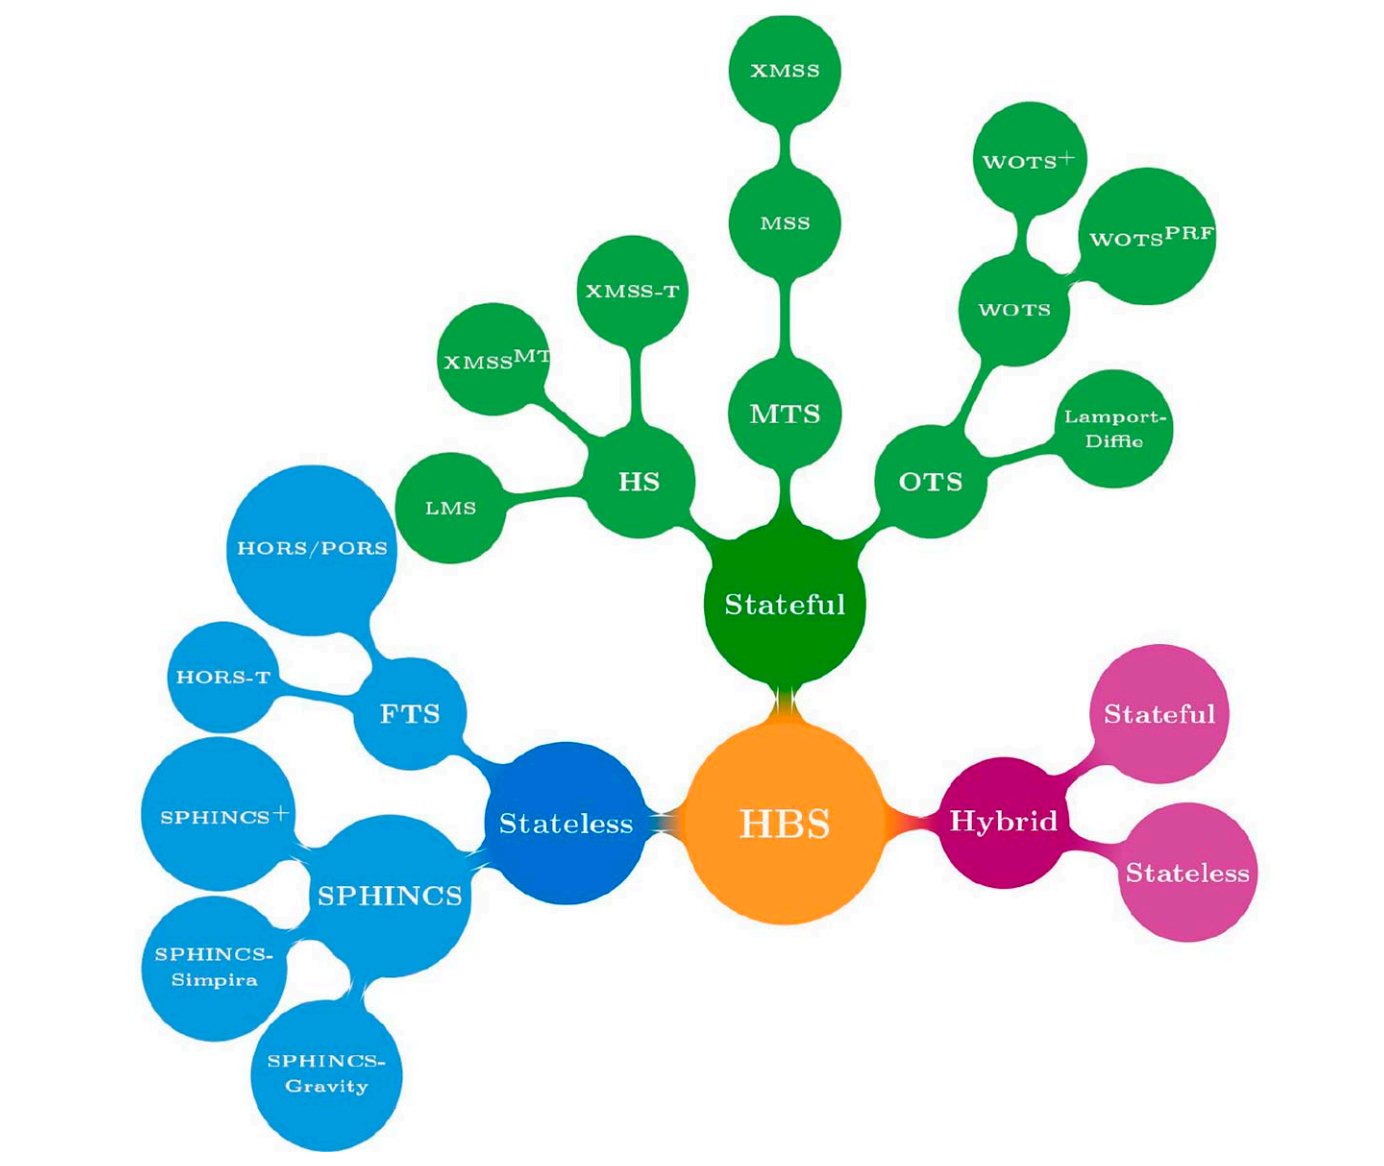
\includegraphics[width=1\textwidth]{Immagini/20240909_HBS.png}
    \caption{Tassonomia e ramificazione dei sistemi di firma \textit{Hash Based}. Fonte: \cite{iot-hashbasedpqc}}
\end{figure}